\documentclass{article}

% Language setting
% Replace `english' with e.g. `spanish' to change the document language
\usepackage[polish]{babel}

% Set page size and margins
% Replace `letterpaper' with `a4paper' for UK/EU standard size
\usepackage[a4paper,top=2cm,bottom=2cm,left=3cm,right=3cm,marginparwidth=1.75cm]{geometry}

% Useful packages
\usepackage{graphicx}
\usepackage{polski}
\usepackage[utf8]{inputenc}
\usepackage{amsmath}
\usepackage{graphicx}
\usepackage[colorlinks=true, allcolors=blue,unicode]{hyperref}
\usepackage{courier}
\usepackage[T1]{fontenc}
\usepackage{lastpage}
\setlength\parindent{24pt}
\usepackage{fancyhdr}
\pagestyle{fancy}
\fancyhead[L]{Sprawozdanie końcowe}
\fancyhead[C]{}
\fancyhead[R]{Kamil Fryszkowski, Oskar Biwejnis}
\cfoot{\thepage/\pageref{LastPage}}


\title{Sprawozdanie końcowe z projektu w języku Java}
\author{Kamil Fryszkowski, Oskar Biwejnis}


\begin{document}
\maketitle
\thispagestyle{fancy}

\section{Cel projektu} 
Celem projektu było napisanie w dwuosobowym zespole programu w języku Java posiadającego graficzny interfejs użytkownika, zbudowany przy użyciu technologii JavaFX, pozwalającego: generować na podstawie danych parametrów albo czytać z pliku graf i wyświetlać jego reprezentacje graficzną, także sprawdzać jego spójność algorytmem BFS oraz obliczać najkrótsze ścieżki pomiędzy danymi punktami za pomocą algorytmu Dijkstry. Miało to nas nauczyć podstaw projektowania GUI, tego jak sprawić aby komunikacja programu z użytkownikiem była efektowna oraz współpracy w pisaniu kodu na zdalnym repozytorium w systemie kontroli wersji GIT.


\section{Struktura programu}
\begin{figure}[htp]
\centering
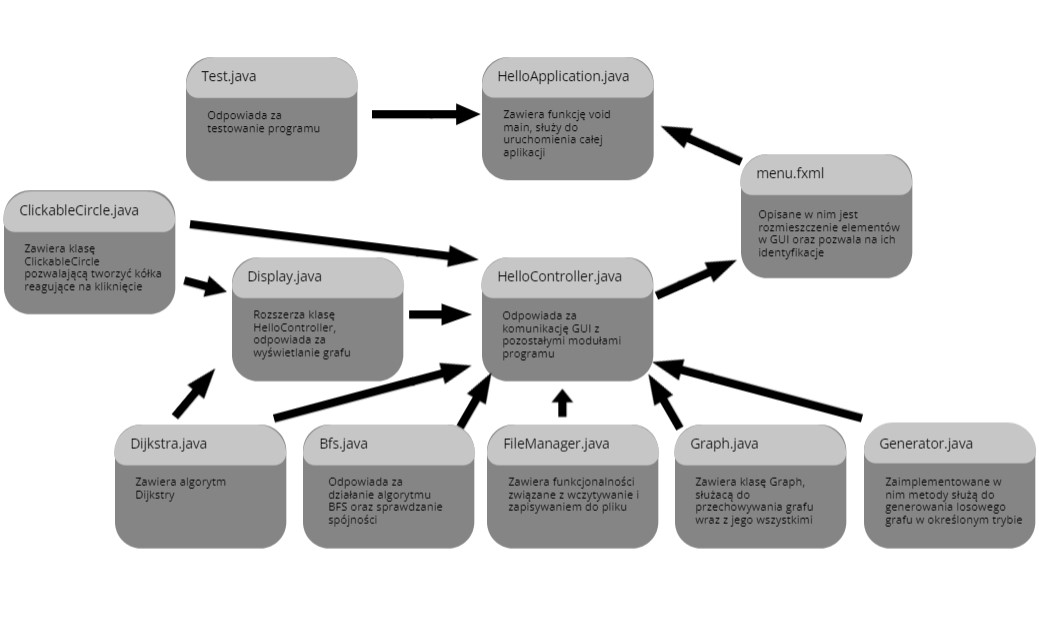
\includegraphics[width=0.9\textwidth]{Screenshot_590.jpg}
\caption{\label{fig:mod}Graficzna reprezentacja struktury programu (opracowanie własne)}
\end{figure}
\begin{itemize}
    \item \texttt\footnotesize{HelloApplication.java} odpowiada za odpowiednie uruchomienie programu, uruchamianie testów i wczytanie sceny
    \item \texttt\footnotesize{Test.java} zawiera testy metod generujących graf, zapisujących i wczytujących plik, BFSa oraz Dijkstry.
    \item \texttt\footnotesize{menu.fxml} to plik zawierający w sobie wygląd GUI
    \item \texttt\footnotesize{HelloController.java} to plik który steruje całym GUI
    \item \texttt\footnotesize{Display.java} to plik, który zawiera metody wykorzystywane przy sterowaniu GUI. Powstał po to, aby \texttt\footnotesize{HelloController.java} był krótszy i czytelniejszy.
    \item \texttt\footnotesize {ClickableCircle.java} dziedziczy po standardowej klasie \texttt\footnotesize{Circle} oraz zawiera on w sobie definicje wyświetlanych w GUI wierzchołków
    \item \texttt\footnotesize{Dijkstra.java} zawiera metody pozwalające na szukanie najkrótszych ścieżek
    \item \texttt\footnotesize{BFS.java} zawiera metody pozwalające na sprawdzenie czy graf jest spójny
    \item \texttt\footnotesize{FileManager.java} zawiera metody które wczytują lub zapisują graf do/z pliku
    \item \texttt\footnotesize{Graph.java} zawiera definicje przechowywania grafu
    \item \texttt\footnotesize{Generator.java} zawiera metody generujące graf
    
\end{itemize}

\pagebreak


\section{Przykładowe wywołania programu}



\subsection {randWeightMode}

 \begin{figure}[htp]
\centering
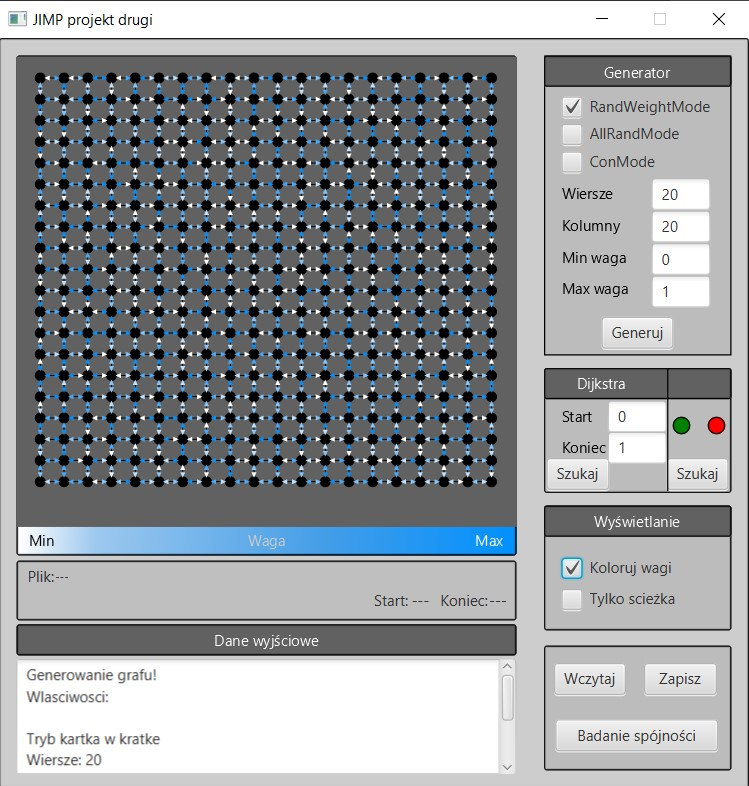
\includegraphics[width=1\textwidth]{Screenshot_582.jpg}
\caption{\label{fig:mod}Graf wygenerowany w trybie losowych wag}
\end{figure}
\pagebreak
 
 


\subsection{allRandMode}

 \begin{figure}[h]
\centering
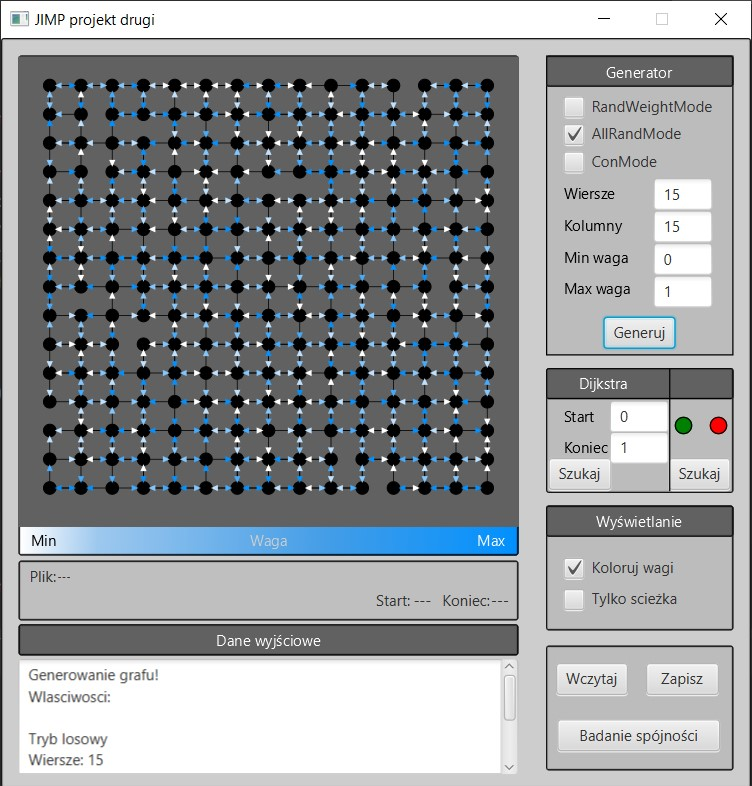
\includegraphics[width=1\textwidth]{Screenshot_583.jpg}
\caption{\label{fig:mod}Graf wygenerowany w trybie całkowicie losowym}
\end{figure}
\pagebreak


\subsection{conMode}

\begin{figure}[h]
\centering
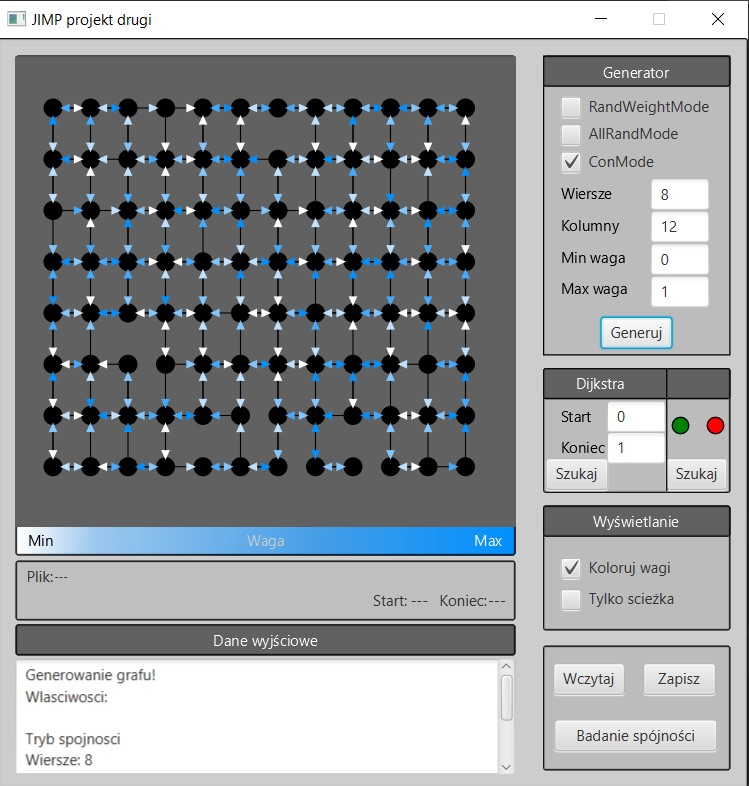
\includegraphics[width=1\textwidth]{Screenshot_584.jpg}
\caption{\label{fig:mod}Graf wygenerowany w trybie spójności}
\end{figure}
\pagebreak

\subsection{loadMode}

 \begin{figure}[h]
\centering
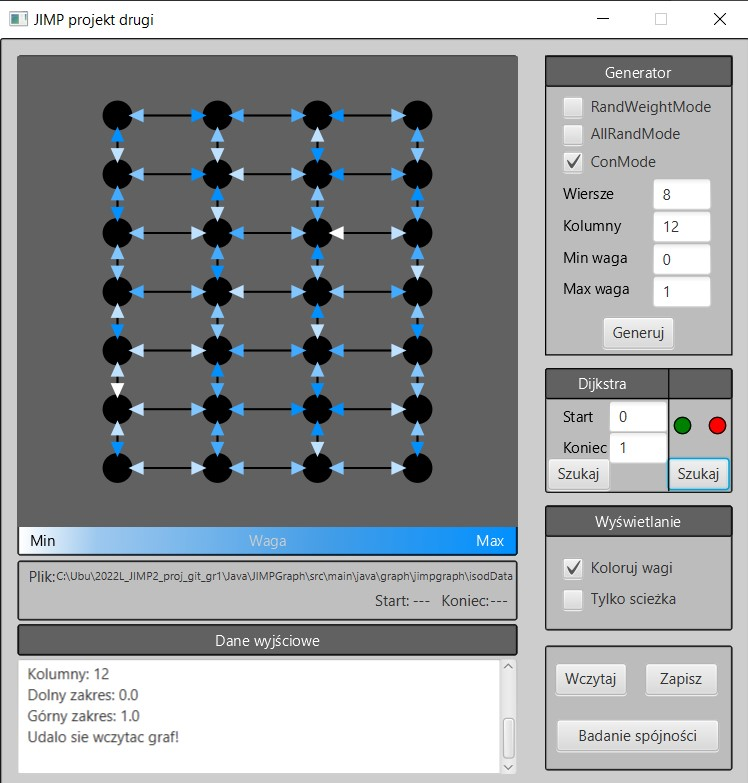
\includegraphics[width=1\textwidth]{Screenshot_585.jpg}
\caption{\label{fig:mod}Wczytany graf z plików z Isod}
\end{figure}
\pagebreak
\subsection{Dijkstra}

 \begin{figure}[h]
\centering
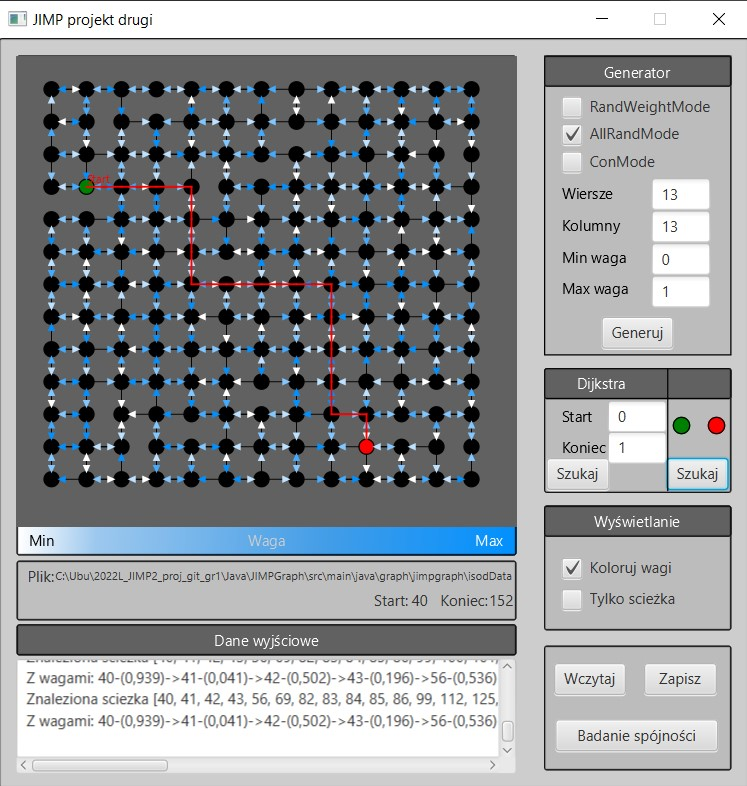
\includegraphics[width=1\textwidth]{Screenshot_586.jpg}
\caption{\label{fig:mod}Wyświetlanie wyniku algorytmu Dijsktry}
\end{figure}
\pagebreak

\begin{figure}[h]
\centering
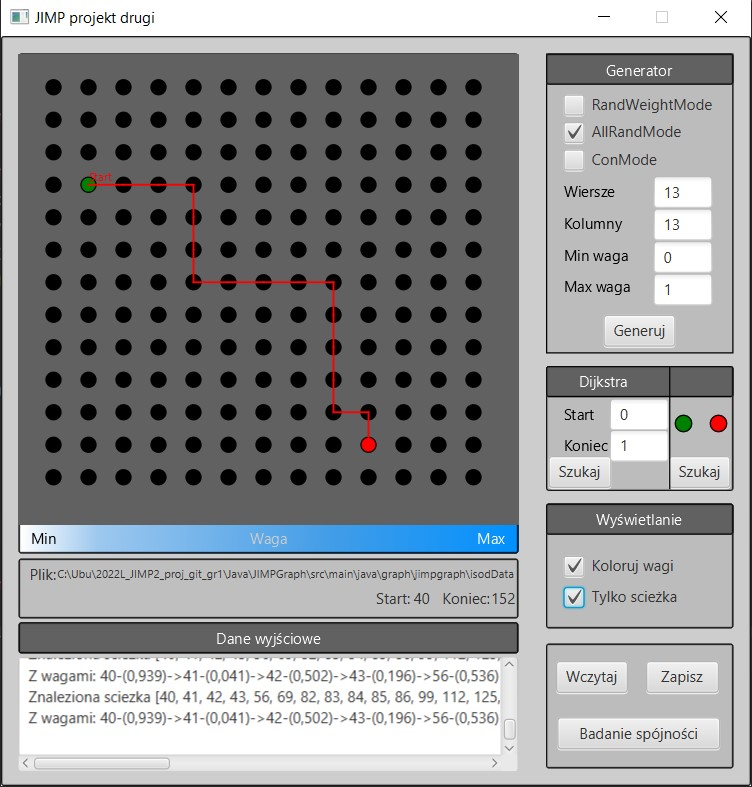
\includegraphics[width=1\textwidth]{Screenshot_587.jpg}
\caption{\label{fig:mod}Włączona opcja pokazująca jedynie ścieżkę}
\end{figure}
\pagebreak









\section{Zmiany w ostatecznej wersji względem pierwotnej}
Zmianie uległ schemat klas oraz zawartości poszczególnych klas
\begin{itemize}
    \item \texttt{\footnotesize app.java} zostało zmienione w trzy osobne klasy, to znaczy \texttt{\footnotesize HelloAplication.java Display.java HelloController.java}.
    
    \item \texttt{\footnotesize Gui.fxml} zmieniło nazwę na \texttt{\footnotesize menu.fxml}.
    
    \item \texttt{\footnotesize Generator.java} nie zawiera tak jak w specyfikacji struktury grafu. Do tego celu została stworzona osobna klasa \texttt{\footnotesize Graph.java}.
    
    \item \texttt{\footnotesize File.java} zmieniło nazwę na \texttt{\footnotesize FileManager.java} ponieważ używaliśmy standardowej klasy \texttt{\footnotesize File} by otworzyć konkretny plik.
    
    \item Powstała nowa klasa \texttt{\footnotesize ClickableCircle.java}, która dziedziczy po standardowej klasie \texttt{\footnotesize Cricle}.
\end{itemize}

\section{Podsumowanie i wnioski}
 Projekt można uznać za zakończony, a jego finalną wersję ocenić pozytywnie. Nauka, w miarę systematyczna praca, wspólna komunikacja oraz wyciąganie odpowiednich wniosków pozwoliły stworzyć program, który niemal całkowicie spełnia założenia jakie sobie postawiliśmy. \\ 
W programie pojawiło się kilka mniej udanych rozwiązań, przede wszystkim testy nie zostały napisane przy pomocy jUnit, a pokazywanie grafu skalowało się do określonej wielkości okna, przez co duże grafy były tak małe że aż niewidoczne. Cała reszta to kosmetyczne kwestie nie wpływające na samą funkcjonalność, czyli sporadyczna, miejscowa niedokładność lub niespójność formatowania kodu. \\ 
Gdybyśmy mieli pisać ten projekt jeszcze raz, to postaralibyśmy się stworzyć widok grafu taki, żeby nawet przy bardzo dużych rozmiarach był widoczny lub możliwy do przybliżenia. Postaralibyśmy się również, aby nie zajmować niepotrzebnie pamięci dla wierzchołków, które nie istnieją, to znaczy powyżej pierwszego wiersza i tym podobnych. Spróbowalibyśmy również napisać cały program w metodyce TDD, koniecznie z wykorzystaniem jUnit (powodem dlaczego od razu nie korzystaliśmy z tej metodyki jest fakt, że to była nasza pierwsza styczność z tworzeniem aplikacji z interfejsem graficznym).
Porównując projekt do poprzedniego, to znaczy aplikacji konsolowej w języku C zauważiliśmy, że jest dużo mniej zmian w porównaniu do specyfikacji. Uważamy, że wynika to z prostego faktu, że de facto tworzyliśmy bardzo podobny program wykorzystując jedynie inny język programowania, jakim jest JAVA, a sam trzon aplikacji opiera się na tych samych zależnościach.

\section{Przebieg współpracy}

Współpracę można ocenić pozytywnie. Dzięki jasno ustalonym wymaganiom, które sobie określiliśmy w specyfikacjach, praca nad programem obyła się bez większych problemów. Komunikacja przebiegała sprawnie od samego początku. Równomiernie podzieliliśmy zadania w zespole i na biężąco informowaliśmy siebie nawzajem o postępach. \\
Pracowaliśmy z pomocą systemu kontroli wersji GIT wykorzystując repozytorium znajdujące się na Projektorze. Każdy z nas miał swoją własna gałąź, na której pracował, a po dokonaniu weryfikacji kodu przez drugą osobę, zmiany były dodawane do gałęzi głównej.


\end{document}